\newcommand{\scaltex}{Scaltex's Latex Projection}
 
 
\chapter{Einleitung}\label{}
 
\section{Motivation}\label{}
 
Die Erstellung von qualitativ hochwertigen (wissenschaftlichen) Dokumenten ist keine einfache Sache. Das Computerzeitalter konnte zwar schon viel verbessern, aber es gibt noch immer Situationen, in denen die Dokumentenerstellung sehr mühselig werden kann.

 
Zum einen kostet es u.U. sehr viel Zeit, Querreferenzierungen im Dokument zu pflegen und konsistent zu halten. Hierfür hat insbesondere LaTeX eine solide Lösung, jedoch stößt man auf der Meta-Ebene (der LaTeX Code selbst) wieder auf das Problem. Beispiel: Man definiert ein Label und referenziert an anderen Stellen darauf. Wird das Label irgendwann umbenannt (weil sich z.B. die Überschrift geändert hat), muss es an allen referenzierten Stellen auch umbenannt werden (klassisches Refactoring) -- und das geschieht leider nicht automatisch.

 
Zum anderen verstehen die Anwendungen oft nur die Domäne „Dokument“, wenn man z.B. chemische Formeln zeichnen will, müssen diese über externe Ressourcen hinzugefügt werden. Dabei gibt es keinen wirklichen Zugriff mehr auf die Meta-Informationen, die eigentlich durch das Domänenmodell -- die chemische Formel -- mitgeliefert wird. Das kann wiederum zu inkonsistenten Dokumenten führen. Wenn z.B. nachträglich an der chemischen Formel etwas geändert wird und nur die Abbildung von Benutzer aktualisiert wurde, dann sind u.U. die Verweise (z.B. auf die Masse des chemischen Moleküls) in den beschreibenden Sätzen nicht mehr korrekt. Es fehlt das semantische Verständnis seitens des Dokuments, es weiß also nicht, was die chemische Formel zu bedeuten hat.

 
Zudem liegt hinter keinem derzeit verfassten Dokument ein echtes/sauberes \emph{Metamodell}. Das heißt ein Modell, welches eine Struktur vorschreibt, wann welche Dokumentbestandteile zulässig sind. Dies kann einen Dokumentenverfasser dabei helfen, ein Dokument (wie z.B. ein Paper der Fraunhofer Gesellschaft) gemäß definierter Vereinbarungen aufzubauen, dabei braucht er kein Wissen über die genaue Vereinbarung und kann dennoch ein formal korrektes Dokument erstellen. Solche Vereinbarungen können z.B. ein Corporate Design oder eine spezielle Reihenfolge von Dokumentelementen sein. Weiterhin kann man ganze Dokumentklassen aus einem solchen Metamodell ableiten; also all jene Dokumente, welchen das gleiche Metamodell übergeordnet ist, gehören somit ganz formal zur gleichen Dokumentklasse. Beispiele für solche Klassen sind: Master-Arbeit, Journal-Paper oder EU-Patent etc.

 
\section{Problemstellung}\label{problemstellung}
 
Aus der Motivation erschließen sich folgende Defizite bzw. Problemfelder in bisherigen Systemen:

 
\begin{enumerate}[(i)]

\item
Mangel an Konsistenz: In bisherigen Textverarbeitungssystemen ist es sehr leicht, Inkostistenzen ins Dokument einzubringen.


\item
Mangel an Domänenwissen: Dokumente „verstehen“ die Konventionen, Konzepte oder Modelle einer Wissenschaft nicht.


\item
Mangel an Semantik: Bedeutungen einzelner Bestandteile eines Dokuments werden oft nicht explizit sichtbar bzw. überhaupt erst verfügbar gemacht.


\item
Mangel an Metamodellierung: Es fehlen\footnote{Oder gehen nicht weit genug, wie z.B. im Falle von LaTeX.} formale Vereinbarungen, die eine Dokumentenklasse ausmachen und dem Benutzer bei der Strukturierung helfen.


\end{enumerate}
 
Das wirft die folgende Frage auf: Kann man ein Autorensystem erschaffen, welches die o.g. Defizite aufhebt?

 
\section{Methode}\label{}
 
In erster Linie soll ein Prototyp entwickelt werden, der einen konkreten Lösungsvorschlag für die Problemstellungen aus Abschnitt \ref{problemstellung} vorlegt.

 
Da ein Prototyp wunderbar untersucht werden kann, ist es möglich, theoretische Ideen besser zu veranschaulichen oder überhaupt erst greifbar zu machen. Zudem können unterschiedliche Anwendungsfälle demonstiert werden, um potentiellen Interessenten dieser Technologie Anschauungsmaterial zu liefern. Die Entwicklung eines Protoypen macht bei dieser Masterarbeit Sinn, da am Prototypen:

 
\begin{itemize}

\item theoretische Konzepte aufgezeigt und empirisch validiert\footnote{Funktioniert das Konzept richtig?} werden können, und
\item leicht Anwendungsfälle ausprobiert werden können, um die praktische Tauglichkeit der Softwarearchitektur zu verifizieren\footnote{Verifikation prüft ob ein System richtig gebaut ist. Oder im Falle von Dokumenten: Ist das Dokument zu einer Spezifikation konform?}.
\end{itemize}
 
\section{Anforderungen}\label{}
 
Bei den Anforderungen an den Prototypen kann man schon konkreter in Richtung Implementierung blicken. Hier die Basisanforderungen, um die Problemstellungen zu lösen:

 
Die kleinste Einheit im System ist das \emph{Dokumentelement}. Beispiele für Dokumentelemente sind: Abschnitte, Absätze, Tabellen, Abbildungen, Fußnoten, etc.

 
Dokumentelemente sollen in der Lage sein, konkretes „lebendinges“ Domänenwissen zu beinhalten. Das heißt, dass z.B. eine Zeichnung eines chemischen Moleküls im Hintergrund tatsächlich auf einem formalen Molekülmodell basiert.

 
Reichhaltige Verweisungen unter den Dokumentelementen sollen möglich sein. Das heißt, dass z.B. das formale Modell des Moleküls anderen Dokumentelementen weitere (u.U. berechnete) Informationen bereitstellen kann.

 
Ein Metamodell definiert die im Dokument vorkommenden Dokumentelemente formal. Das Dokument selbst soll folglich als Modell (Instanz) aufgefasst werden.

 
Um die Software benutzbar zu machen:

 
\begin{itemize}

\item Es soll ein reaktives System sein, welches sofort auf Eingaben des Benutzers bzw. Veränderungen des Systemzustands reagiert.
\item Es soll also ein „lebendiges“ Dokument werden, d.h. es sollen keine (spürbaren) Kompilierzeiten, um das Dokument zu erstellen, entstehen.
\item Da es in wissenschaftlichen Dokumenten meist zu komplizierten Verweisungen kommt, müssen diese in jedem Fall konsistent gehalten werden. Es soll daher das Verweisvariablen-Refactoring-Problem abgefedert werden.
\item Es soll ein Einheimischer des WWW werden, d.h. Web Standards sind das Ausgabeformat. Sie übernehmen das Setzen des Dokuments, bieten dem Benutzer eine Editierschnittstelle, ermöglichen Kollaboration und bieten eine ubiquitäre Wissensrepräsentation.
\end{itemize}
 
Durch einige dieser Anforderungen gewinnen wir implizit einen Projektionseditor und sogar Potential für ein Dokument „Query Interface“.

 
\section{Idee}\label{}
 
Im Vordergrund stand die Idee, meine Bachelorarbeit so weiter zu entwickeln, dass Dokumente in einem Struktureditor oder Projektionseditor verfasst werden können und mit domänenspezifischen Dokumentelementen interagiert werden kann.

 
In diesem Kapitel wird also kurz die prinzipielle Idee umrissen, wie man die Problemstellung unter den gegebenen Anforderungen lösen könnte.

 
Grundsatz der Idee ist, dass jedes Dokumentelement auf ein Aktor abgebildet wird. Ein Aktor kann Nachrichten senden und empfangen, zudem kapselt er einen Zustand und ein Verhalten.

 
Aktoren können, ebenso wie ein Dokument, hierarchisch angeordnet werden. Das heißt ein Aktor kann Kinder und Geschwister haben. Diese Anordnung ergibt eine baumartige Graphenstruktur, worin ein Aktor einem Knoten entspricht und eine Referenz\footnote{Über eine solche Aktor Referenz können Nachrichten an andere Aktoren übermittelt werden.} auf einen anderen Aktor einer Kante.

 
Diese Baumstruktur kann als abstrakter Syntaxbaum (AST) der Dokumentenstruktur aufgefasst werden. Der AST kann als ein Modell für ein Dokument aufgefasst werden. Dies wird auf Abbildung \ref{idee} veranschaulicht. Zudem kann mit Hilfe eines AST ein Struktureditor umgesetzt werden. Der hier mit den Aktoren umgesetzte AST könnte als „reaktiver AST“ bezeichnet werden, da er dank der Aktoren (quasi gratis) besondere Eigenschaften erhält:

 
\begin{itemize}

\item Verteilbarkeit, Fehlertoleranz und massive Parallelität. AST kann z.B. auf ein Cluster gebracht werden, z.B. zur Kompilierung des Dokuments in „der Cloud“; Anwendung von MapReduce auf Dokument oder Dokumentenserie; Jeder Aktor ist autonom, d.h. z.B. asynchrone Datanbankzugriffe oder schnelle Reaktionszeiten auf Änderungen.
\item Möglichkeit zum Query Interface ausgebaut zu werden. Das Dokument bzw. Dokumentelement kann auf Nachrichten reagieren. Beispielsweise zur Aggregation neuer Informationen.
\item Möglichkeit mit anderen (Aktoren-) Systemen (z.B. Dokumenten) zu interagieren. Beispielsweise via Akka Remoting Protokoll oder Anbindung an REST-Schnittstellen.
\end{itemize}
 
\begin{figure}[h!]
\centering
\advance\leftskip-2.5cm
\fbox{ 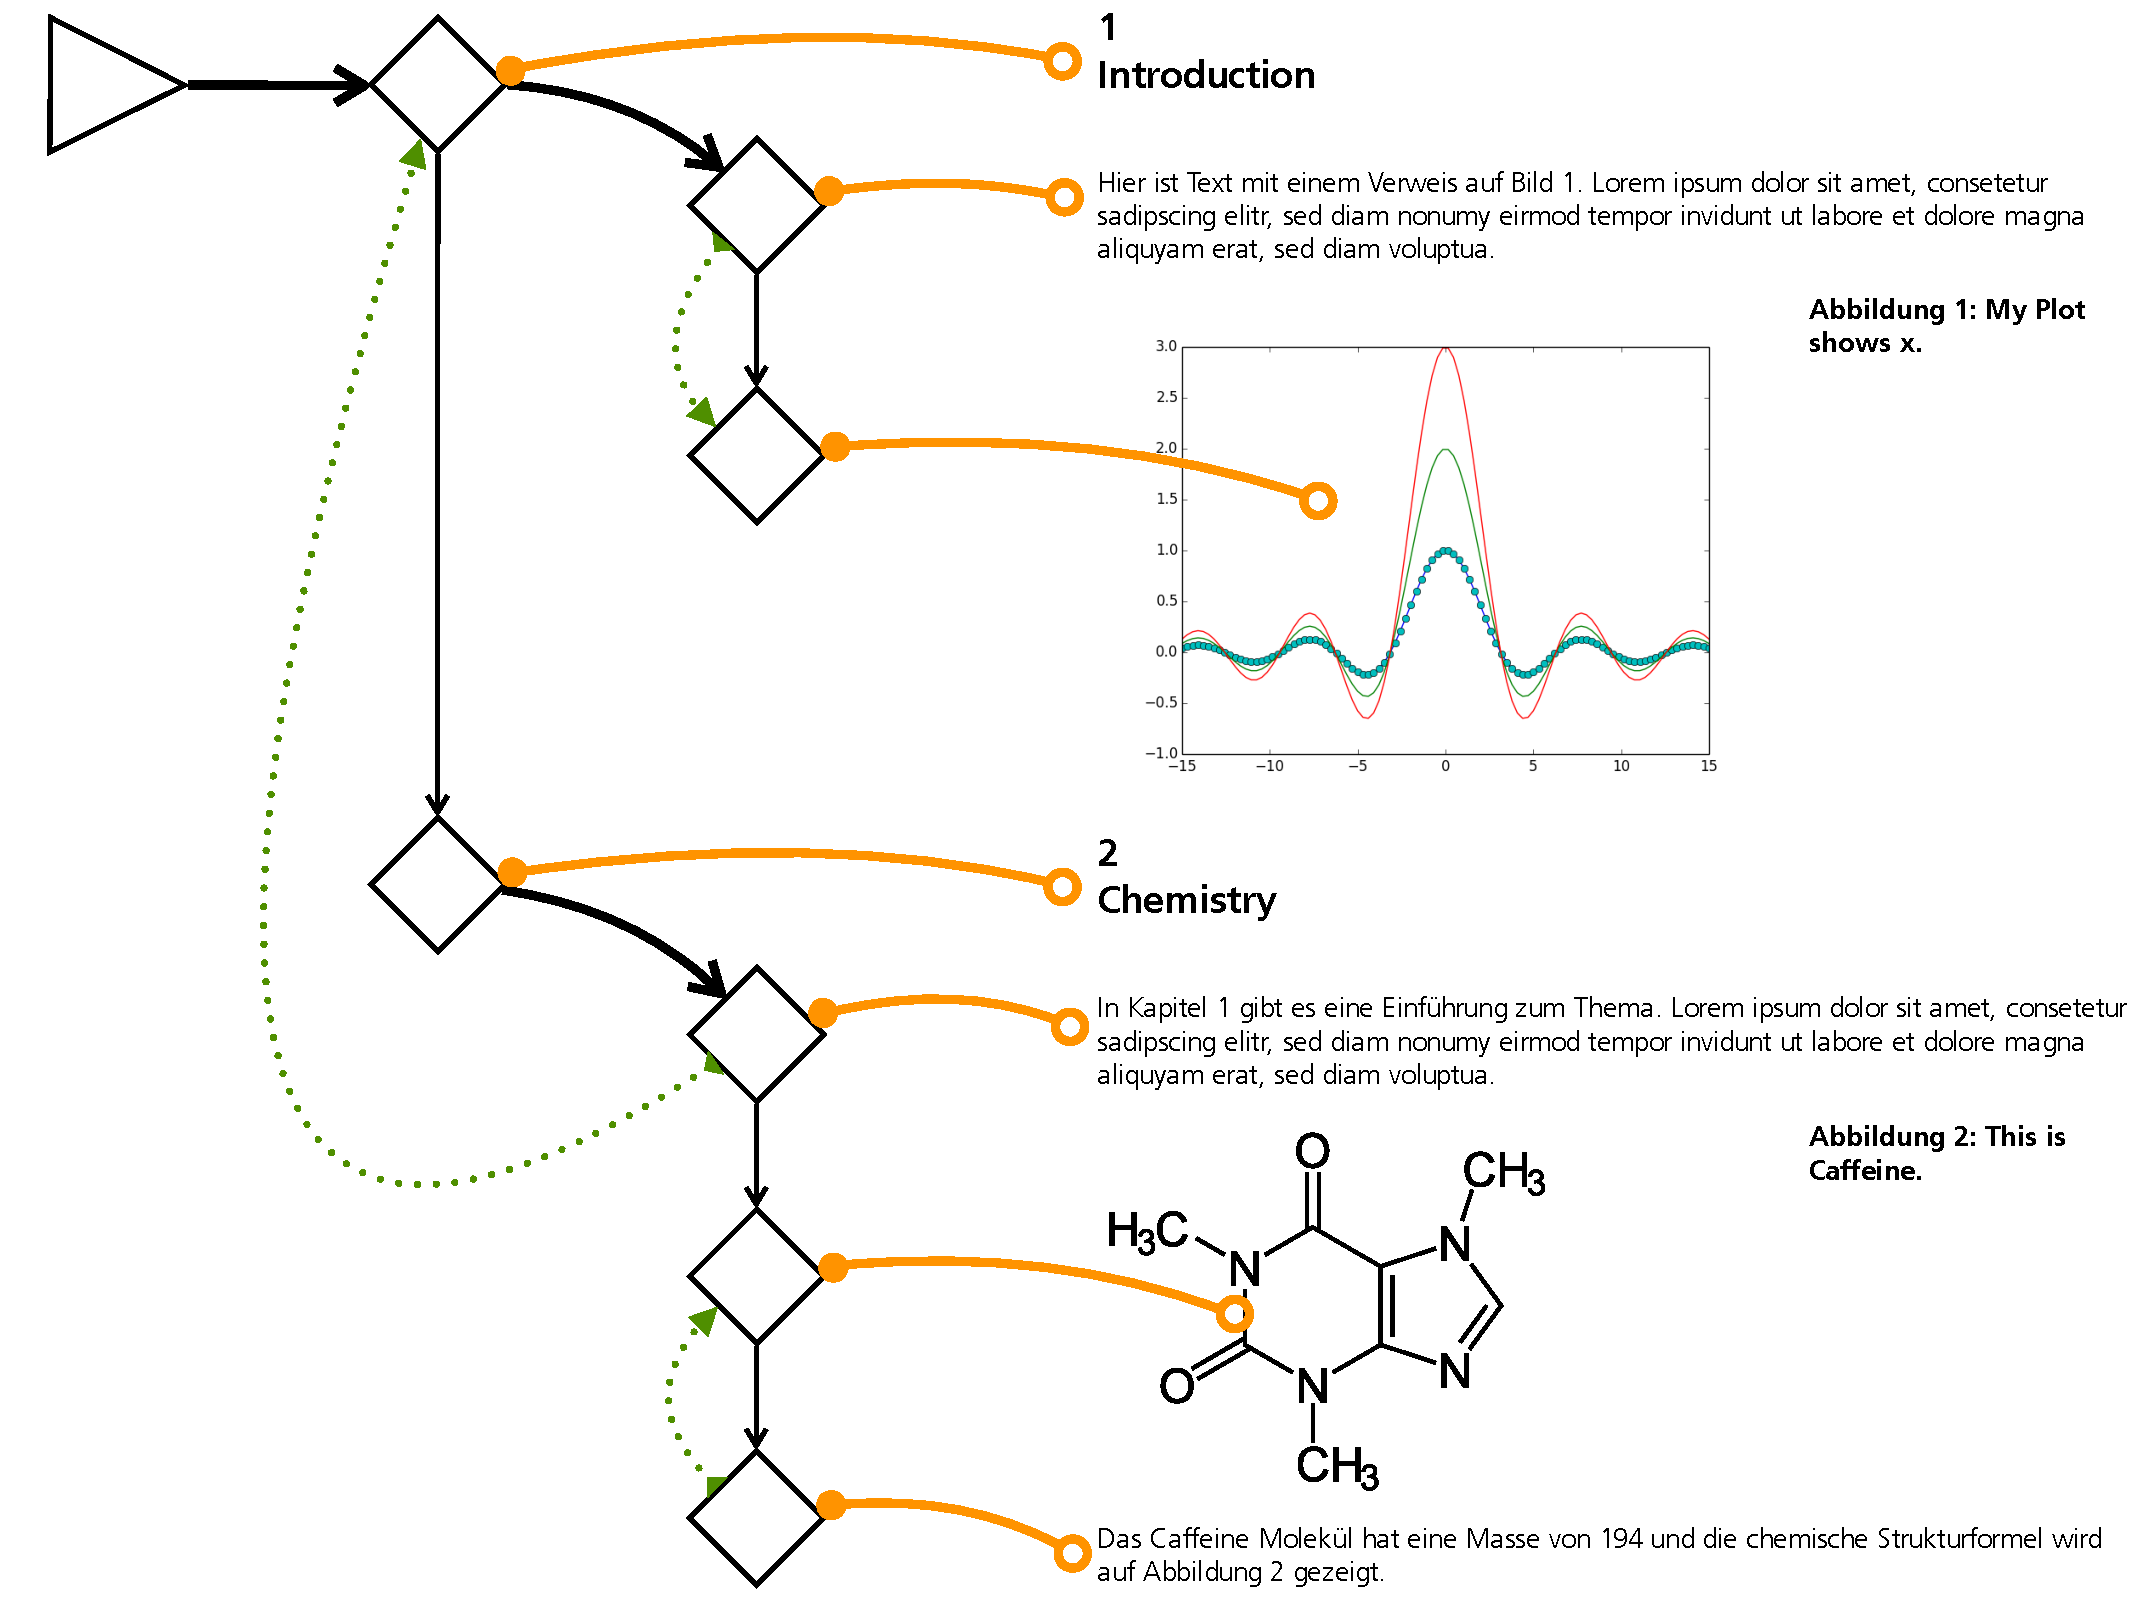
\includegraphics[width=1.45\textwidth]{figures/idee.svg.pdf} }
\caption{ Modell für ein Dokument. Jeder Aktor (Raute) repräsentiert ein Dokumentelement. Die Aktoren kennen sich (graue Pfeile) und spannen somit einen Graphen auf. Die Aktoren können Nachrichten (grüne Pfeile) austauschen, z.B. um Benummerungen aufzulösen. }\label{idee}
\end{figure}
 
\section{Szenario}\label{}
 
\section{Fragen von wissenschaftlichem Interesse}\label{}
 
Bereiche in denen (wiss.) Fragestellungen durch den Prototypen beantwortet werden können:

 
\begin{itemize}

\item
Modellgetriebene Software-Entwicklung: Ist es sinnvoll Dokumente als Modell aufzufassen? Wie könnte eine sinnvolle Modellierung von Dokumenten aussehen? Gibt es ein gemeinsames Metamodell?


\item
Programmiersprachen, Compilerbau: Kann ein Aktorsystem verwendet werden, um einen abstrakten Syntaxbaum zu implementieren? Taugt dieser abstrakte Syntaxbaum als sinnvolle Architekturgrundlage für einen Projektionseditor, und damit auch als Code Generator?


\item
Knowledge Engineering / Management; Semantik, Ontologie: Brauchen wir mehr explizite Semantik innerhalb von Dokumenten? Ergeben sich Vorteile, wenn diese Semantik direkt vom Autor transportiert wird? Ist es möglich, dass sich Dokumente zu einem gewissen Grad selbst verifizieren\footnote{Verifikation prüft ob ein System richtig gebaut ist. Oder im Falle von Dokumenten: Ist das Dokument zu einer Spezifikation konform?} und damit konsistenter machen?


\item
Bibliotheks- und Informationswissenschaften: Gibt es eine allgemeingültige Taxonomie für wiss. Publikationen?


\end{itemize}
 
\chapter{Theorie}\label{}
 
In diesem Kapitel werden theoretische Konzepte erarbeitet.

 
\section{Modellbegriff}\label{}
 
\begin{quote}
 Modellierung ist das uns angeborene Verfahren, das komplexe Universum auf eine überschaubare Welt zu reduzieren. Indem wir sichtbare und unsichtbare Phänomene auf Begriffe abbilden und nur noch mit diesen umgehen, wird die Gesamtzahl der zu betrachtenden Gegenstände beherrschbar[...] \citep[S.~7]{Ludewig}
\end{quote}
 
Gerade auch in der Wissenschaft spielen Modelle die zentrale Rolle, denn „Das Resultat einer Forschung ist in jedem Falle ein Modell, eine Theorie.“ \citep[S.~8]{Ludewig} Warum sollte man also nicht den Weg ganz konsequent gehen, und ebenfalls die wissenschaftliche Dokumentation selbst als Modellierung betrachten? Warum sollte das Dokument selbst nicht Modelle aus einer Wissenschaft bereitstellen? Das heißt, dass eine Wissenschaftlerin bzw. ein Wissenschaftler seine Modelle direkt im Dokument verwenden kann?

 
\subsection{Modellmerkmale}\label{modellmerkmale}
 
In \citep[S.~9]{Ludewig} ist eine griffige Zusammenfassung der drei zwingenden Merkmale die nach \citep{Stachowiak} vorliegen müssen, um als Modell zu gelten, aufgeführt. Diese werden hier sinngemäß zusammengefasst und durch Abbildung \ref{modell} veranschaulicht:

 
\begin{enumerate}

\item Abbildung: Ein Modell ist immer ein Abbild eines Originals. Die Abbilder können beliebig geartet sein, d.h. das Modell muss dem Original äußerlich nicht ähneln. Das Original auf welches sich das Modell bezieht, kann neben natürlichen Objekten auch künstlich, geplant oder vermutet sein.
\item Verkürzung: Ein Modell erfasst nicht alle Merkmale des Originals. Durch Verkürzung fallen Attribute weg, diese werden übergangen oder präteriert genannt. Das Modell kann jedoch zusätzliche Attribute haben, die so im Original nicht vorkommen, diese werden überflüssig oder abundant genannt.
\item Pragmatismus: Ein Modell muss einen Sinn haben, um unter bestimmten Fragestellungen das Original ersetzen können. Das heißt, es wird das Modell statt des Originals untersucht, um daran die Nützlichkeit für eine Zielgruppe (für wen, wann, wozu?) festzustellen.
\end{enumerate}
 
\begin{figure}[h!]
\centering
\advance\leftskip-2.5cm
\fbox{ 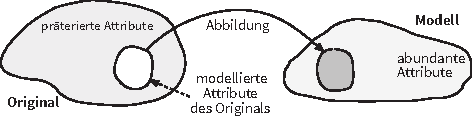
\includegraphics[width=1.45\textwidth]{figures/modell.svg.pdf} }
\caption{ Schematische Zeichnung der Original-Modell-Beziehung. Entnommen aus (Ludewig, 2002, S. 9). }\label{modell}
\end{figure}
 
\subsection{Modell eines Dokuments}\label{dokumentModell}
 
Bevor ein passendes Modell für Dokumente gefunden werden kann, muss man sich bewusst sein dass es dem Abbildungsmerkmal, Verkürzungsmerkmal und dem pragmatischen Merkmal, welche in Kapitel \ref{modellmerkmale} beschrieben sind, genügen muss.

 
Das Original ist in jedem Fall ein gesetztes statisches Dokument, z.B. ein auf Papier gedrucktes Buch oder ein (wiss.) Bericht im PDF-Dateiformat.

 
Dort interessieren uns als Autor in erster Linie aber nur die wirklich inhaltstragenden Attribute des Originals. Auf einer höheren Abstraktionsebene entsprechen diese den Dokumentelementen, wie z.B. Abschnitte, Absätze, Abbildungen etc. Im Falle von z.B. Abschnitten ist nur der Titel maßgeblich, die Benummerung kann auch erst später (durch Berechnung) hinzugefügt werden. Das heißt hier wäre der Titel ein Attribut welches vom Original in das Modell abgebildet wird; die Benummerung wäre jedoch ein abudantes Attribut welches erst innerhalb des Modells erstellt wird. Layoutinformationen, Schriftarten oder Papiersorte spielen dafür keine Rolle und können somit weggelassen werden.

 
Wenn der Autor an seinem Dokument arbeitet, dann stets über das Modell, wo er sich ausschlißlich auf die Dokumentelemente konzentrieren kann. Das Modell kann präskriptiv sein, d.h. aus dem Modell kann wieder ein Original entspringen.

 
Hier wird der abstrakte Syntaxbaum als Modell für das Dokuments dienen, indem jedes Dokumentelement aus ein Knoten des abstrakten Syntaxbaum aufgefasst wird. Mehr zum abstrakten Syntaxbaum in Abschnitt \ref{ast}.

 
\subsubsection{Beweis}\label{}

 
\begin{itemize}

\item
Abbildungsmerkmal: Der abstrakte Syntaxbaum („das Modell“) ist z.B. ein Abbild eines gedruckten Buches, da Dokumentelemente als Knoten im Syntaxbaum vorkommen.


\item
Verkürzungsmerkmal: Nur die Attribute aus dem Original werden modelliert, die den maßgeblichen Inhalt des Dokuments transportieren (z.B. Text). Diese Inhalte werden als Dokumentelemente modelliert.


\item
Pragmatischen Merkmal: Der Autor greift auf das Modell zurück, um daran die herausgelößten und essentiellen Dokumentelemente zu untersuchen bzw. zu manipulieren.


\end{itemize}
 
Alle Bedingungen für den Modellbegriff nach \citep{Stachowiak} sind erfüllt. ■

 
\section{Abstrakter Syntaxbaum}\label{ast}
 
In diesem Abschnitt werden die prinzipiellen Eigenschaften von abstrakten Syntaxbäumen, kurz AST, beschrieben.

 
Laut \citep{Aho} ist der AST eine Datenstruktur, die von einem Übersetzer als Zwischenrepräsentation eines Quellcodes generiert wird. Er repräsentiert die hierarchische syntaktische Struktur eines Programms. Aus einer solchen Zwischenrepräsentation wird schlussendlich das Zielprogramm generiert.

 
Wärend der Syntaxanalyse (parsing) werden Syntaxbaum-Knoten erstellt, welche wiederum signifikate Programmkonstrukte repräsentieren. Die Kinder des Knoten sind die bedeutungstragenden Komponenten des Konstrukts. Beispielsweise (s. Abb. \ref{ast}): Gegeben ist ein AST für einen Ausdruck (expression), dann repräsentiert jeder innere Knoten einen Operator und die Kinder des Knoten sind die Operanden. Man beachte jedoch, dass Syntaxbäume für beliebige Konstrukte erstellt werden können und nicht auf Ausdrücke beschränkt sind. Jedes Konstrukt ist durch einen Knoten repräsentiert, dessen Kinder semantisch bedeutungsvolle Komponenten des Konstruktes sind. Durch fortschreitende Analyse können Informationen vom Übersetzer zu den Knoten als Attribute hinzugefügt werden. (ebd.)

 
\begin{figure}[h!]
\centering
\advance\leftskip-2.5cm
\fbox{ 
\includegraphics[width=1.45\textwidth]{figures/ast.svg.pdf} }
\caption{ Abstrakter Syntaxbaum für den Ausdruck 9-5+2. Entnommen aus (Aho, 2007, S. 70). }\label{ast}
\end{figure}
 
\subsection{Allgemeine Implementierung}\label{}
 
Wenn ein Operator, also ein innerer Knoten, beliebig viele Operanden, also Kinder des Knoten, haben darf, spricht man von einem n-stelligen bzw. n-ary AST. \citep{Edwards} Eine solche Struktur ist auf Grafik \ref{astimpl} veranschaulicht.

 
\begin{figure}[h!]
\centering
\advance\leftskip-2.5cm
\fbox{ 
\includegraphics[width=1.45\textwidth]{figures/astimpl.svg.pdf} }
\caption{ Generellste Implementierung eines AST. Entnommen aus (Edwards, 2003). }\label{astimpl}
\end{figure}
 
\subsection{Übertragung auf den Prototypen}\label{}
 
Die zentrale Struktur des hier vorgestellten Prototyps ist ebenfalls ein abstrakter Syntaxbaum. Das ist legitim, da Syntaxbäume beliebige Konstrukte repräsentieren können. Jedoch handelt es sich nicht ausschließlich um eine Datenstruktur, da Aktoren als die Baum-Knoten fungieren und Aktoren neben der reinen Datenhaltung auch auf Nachrichten reagieren können. Man könnte quasi davon sprechen, dass der abstrakte Syntaxbaum in dem hier vorgestellten System eine „lebendige Datenstruktur“ ist. Das kann dahingehend von Vorteil sein, da der AST dadurch befähigt ist, selbstständig eine Analysephase durchzuführen.

 
In einer solche Analysephase werden u.U. weitere Informationen zu den Knoten hinzugefügt. Beispiel: Eine Hierarchie von Kapiteln kann während der Analyse die jeweils richtige Benummerung ermitteln und jeder Aktor (also Knoten) speichert sich diese Benummerung intern als Attribut ab.

 
Der Basis Aktor aus Abbildung \ref{metamodell} entspricht quasi 1:1 der generellen Implementierung aus Abbildung \ref{astimpl}. Das hier vorgestellte Metamodell (s. Abschnitt \ref{metamodell_dokument}) beschreibt auch eindeutig einen AST. Die Knoten entsprechen den Aktoren, welche wiederum die einzelnen Dokumentelemente des Dokuments repräsentieren. Dieser AST, gesehen als Programmsyntax, beschreibt somit den hierarchischen Aufbau des Dokuments.

 
Die inneren Knoten, die z.B. Operatoren repräsentieren können, entsprechen hier hierarchiebildenden oder gliedernden Elementen. Diese können (müssen aber nicht) im Dokument sichtbar sein. Beispiele dafür sind z.B. Kapitel, Abschnitte oder die Titelei. Die Kinder dieser Knoten sind bedeutungsvolle Komponenten für den Knoten dahingehend, dass sie entweder weiter die Hierarchie des Dokuments aufspannen und somit das Dokument weiter gliedern oder im Falle von Blättern, die eigentlich inhaltstragenden Elemente sind. Die Blätter müssen auf jeden Fall im Dokument sichtbar sein. Beispiele dafür sind z.B. Absätze oder Abbildungen.

 
\section{Projektionseditoren}\label{}
 
Für gewöhnlich arbeiten Programmierer mit Quellcode-Editoren, das heißt es werden Schriftzeichen direkt in eine Datei geschrieben. Diese Schriftzeichen bilden die konkrete Syntax einer Programmiersprache. Der Editor kann das arbeiten mit Quellcode erleichtern, indem er z.B. die Schlüsselwörter einer Programmiersprache farbig hervorhebt. Um ein Programm aus der Datei zu generieren, muss ein Übersetzer zunächst eine Syntaxanalyse (parsing) durchführen. Bei dieser Analyse wird die Datei in Wörter, die es in der Programmiersprache gibt, zerhackt. Anhand dieser Wörter kann der Übersetzer z.B. eine Baumstruktur aufbauen, um die syntaktische Korrektheit des Programms zu prüfen. Das heißt der Übersetzer kann anhand es Baumes feststellen, ob es sich um ein korrektes Programm handelt. Dann kann aus der, als korrekt befundenen, Baumstruktur der eigentliche Maschinencode erzeugt werden.

 
Projektionseditoren gehen anders vor: Der Editor arbeitet direkt auf dem abstrakten Syntaxbaum (s. Abschnitt \ref{ast}), d.h. der Programmierer editiert nicht mehr eine Datei die durch den Übersetzer in eine Baumstruktur umgewandelt wird, sondern seine editier-Operationen verändern direkt die Baumstruktur des Programms. \citep[S.~68]{Voelter} Nun kann aus der abstrakten Syntax (entspricht der Baumstruktur) eine Variation an konkreten Syntaxen erstellt werden, die sogenannten Projektionen. Diese Projektionen können wieder textuell sein, aber auch grafisch -- jedoch sind diese in ihrer Darstellung deutlich flexibler als bei der parserbasierten Editoren. Eine kurze schematische Grafik (Abb. \ref{parserprojectional}) verdeutlicht den Unterschied zwischen Quellcode-Editoren und Projektionseditoren.

 
Im englischen\footnote{vgl. Wikipedia: \url{http://en.wikipedia.org/wiki/Projectional_editor}} Sprachraum gibt es mehrere Bezeichnungen: structure editor, structured editor oder projectional editor. Man kann diese mit Struktureditor oder Projetkionseditor übersetzten.

 
Die Idee von Projektionseditoren ist nicht neu, bereits 1971 hat Wilfred J. Hansen ein System entwickelt, welches auf solch einem Ansatz beruht. Jedoch haben sich zur damaligen Zeit diese Editor-Formen nicht durchgesetzt, wegen der unzureichenden Benutzerfreundlichkeit. \citep[S.~91]{Gomolka} In heutigen Zeiten (insbesondere mit den fortgeschrittenen Web Standards) sollte es aber möglich sein, einen Benutzerfreundlichen Projektionseditor zu bauen, der die Produktivität und den Komfort erhöht.

 
\begin{figure}[h!]
\centering
\advance\leftskip-2.5cm
\fbox{ 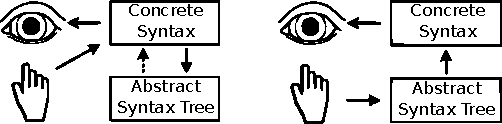
\includegraphics[width=1.45\textwidth]{figures/parserprojectional.svg.pdf} }
\caption{ Parserbasierte Editierung / Quellcode-Edior (links) verglichen mit projektionsbasierter Editierung / Projektionseditor (rechts). Grafiken aus (Voelter, 2013, S. 68) entnommen. }\label{parserprojectional}
\end{figure}
 
\subsection{Übertragung auf den Prototypen}\label{}
 
Der hier vorgestellte Prototyp ist augenscheinlich ein Projektionseditor. Sein Basiskonzept ist Dokumente als ein Modell zu sehen. Und das Modell eines Dokuments erscheint hier in Form eines abstrakten Syntaxbaumes. (s. Kapitel \ref{dokumentModell}) Der Editor arbeitet also „per Design“ als Projektionseditor. Die Projektionen entsprechen einfachen HTML-Templates, die jedem Dokumentelement sein Aussehen verleihen. Werden die Templates ausgetauscht, können ganz andere Repräsentationen bzw. konkrete Syntaxen des vorliegenden abstrakten Syntaxbaumes möglich sein. Beispielsweise kann der Prototyp aktuell neben der „gesetzten“ Web-Ansicht auch noch LaTeX-Code als Projektion anbieten -- das gleiche Dokument in verschiedenen Ansichten oder Projektionen.

 
\section{Metamodellbegriff}\label{}
 
\begin{quote}
 Werden Modelle und Modellbildung selbst zum Gegenstand der Modellierung, so spricht man von Metamodellen. \citep[S.~1]{Strahringer}
\end{quote}
 
\citep{Strahringer} hat versucht den Metamodellbegriff anhand der Sprachstufentheorie der Logik, durch Übertragung auf die Modellierungswelt, zu prägen. \citep[S.~1]{Strahringer} erklärt, dass nach \citep{Buehler} die Sprache drei Funktionen leistet: (1) Darstellung von Sachverhalten, (2) Appell zur Verhaltenssteuerung und (3) Ausdruck von Gefühlen. Für den Metamodellbegriff ist jedoch nur die Darstellungsfunktion interessant. Sprache stellt „ein mögliches Instrument zur Darstellung von Modellen“ (ebd.) dar.

 
\citep[S.~1]{Strahringer} führt fort, dass in der Logik üblicherweise zwischen Objektsprache und Metasprache unterschieden wird. Die Objektsprache ist Gegenstand der Untersuchung. In der Metasprache erfolgt die Untersuchung. Da die Metasprache selbst auch wieder Gegenstand einer Untersuchung werden kann, ist dieses Prinzip rekursiv anwendbar. Um endlose Rekursion zu vermeiden, sollte als oberstes Glied der Kette ein selbstbeschreibendes Metamodell stehen. Beispielsweise die Meta Object Facility (MOF) der OMG\footnote{Definiert in ISO/IEC 19508.} geht so vor, um endlose Meta-Rekursionen zu vermeiden.

 
Wird „die Sprachstufentheorie auf die Modellbildung [...] übertragen, so“ (ebd.) kann im einfachsten Fall ein Metamodell „als ein Modell eines Modells“ (ebd.) beschrieben werden.

 
\begin{quote}
 Wird die Objektsprache, in der das Modell der untersten Stufe formuliert ist, abgebildet in einem Beschreibungsmodell, so handelt es sich um ein Metamodell. \citep[S.~3]{Strahringer}
\end{quote}
 
„Beschreibungsmodelle dienen der systematischen Beschreibung des betrachteten Gegenstandsbereiches und bestehen aus ausschließlich deskriptiven Satzsystemen.“ Das heißt, ein Beschreibungsmodell ist ein Modell welches so formuliert wird, dass es ein Original anschaulich macht bzw. Eigenschaften des Originals sprachlich spezifiziert. Abbildung \ref{metamodellbegriff} veranschaulicht den Zusammenhang von Modell und dessen Metamodell.

 
\begin{figure}[h!]
\centering
\advance\leftskip-2.5cm
\fbox{ 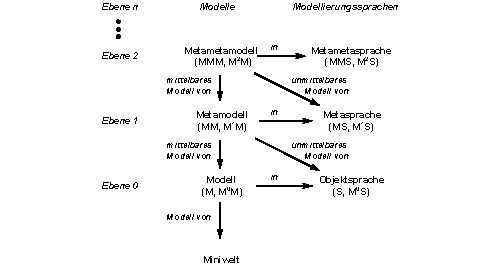
\includegraphics[width=1.45\textwidth]{figures/metamodellbegriff.svg.pdf} }
\caption{ Der sprachbasierte Metamodellbegriff. Die „Miniwelt“ entspricht dem Original. Grafik entnommen aus (Strahringer, 1998, S. 3). }\label{metamodellbegriff}
\end{figure}
 
\subsection{Metamodell des Dokumentmodells}\label{metamodell_dokument}
 
Damit das Modell formal und damit nicht verschwommen spezifiziert ist, brauchen wir ein Metamodell. Das Metamodell schafft somit auf einer abstrakteren Ebene Klarheit über das Modell.

 
Auf Abbildung \ref{docmodell} ist das eigentliche Modell visualisiert. Dieses soll vom Metamodell beschrieben werden.

 
\begin{figure}[h!]
\centering
\advance\leftskip-2.5cm
\fbox{ 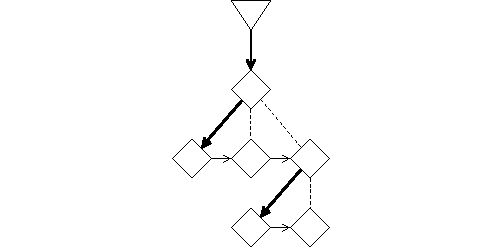
\includegraphics[width=1.45\textwidth]{figures/docmodell.svg.pdf} }
\caption{ Das hier verwendete Dokumentmodell. Das Dreieck symbolisiert die Wurzel. Die Rauten symbolisieren jeweils einen Aktor bzw. ein Dokumentelement. Die stark gezeichneten Pfeile symbolisieren das erste Kind, die gestrichelte Linie symoblisiert die zugehörigen anderen Kinder. Die schwach gezeichneten Pfeile symbolisieren die nächstes Geschwister. Dadurch wird die Dokumenthierarchie aufgespannt. }\label{docmodell}
\end{figure}
 
Abbildung \ref{metamodell} zeigt das Modell welches das Dokumentmodell beschreibt, also das „Metamodell“. In der Mitte liegt der Basis Aktor, dieser hält Referenzen zu seinem ersten Kind und zu seinem unmittelbaren Geschwister. Zudem hält der Basis Aktor Inststanzen aller verfügbaren Dokumentelemente, wovon jedoch immer nur eine aktiv ist. Welche Dokumentelemente verfügbar sind, wird vom Programmierer spezifiziert -- dazu muss er ein Scala Trait (entspricht einem Interface) implementieren und dem Basis Aktor bekannt machen. Man kann sagen, dass er das Metamodell an dieser Stelle (gewollt) verändert. Der Wurzel Aktor hält nochmals alle Topologieinformationen, daher kennt er alle im System vorhandenen Basis Aktoren. Jeder Basis Aktor kennt auch seine zugehörige Wurzel, welche er bei ggf. anstehenden lokalen Topologieveränderungen benachrichtigen muss.

 
\begin{figure}[h!]
\centering
\advance\leftskip-2.5cm
\fbox{ 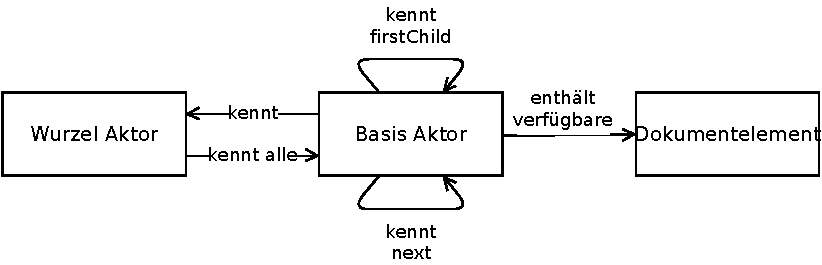
\includegraphics[width=1.45\textwidth]{figures/metamodell.svg.pdf} }
\caption{ Das Metamodell des Dokumentmodells. }\label{metamodell}
\end{figure}
 
\subsubsection{Beweis}\label{}

 
Die Besonderheit bei dem hier entstandenen System ist, dass das Modell gleichzeitig die Sprache ist, in der es modelliert wird. Dies ist möglich, da das System als Projektionseditor designed ist. Die Objektsprache in der das Modell formuliert ist, entspricht somit quasi der Projektion die direkt aus dem abstrakten Syntaxbaum entspringt. Man könnte von einem „Modell-Objektsprache-Dualismus“ sprechen -- es ist gleichzeitig Modell und Objektsprache, je nach Betrachtungspunkt.

 
Das Modell indem wiederum die Objektsprache modelliert ist, muss ein Beschreibungsmodell sein, damit dies einem Metamodell entspricht. Das hier vorgestellte Metamodell spezifiziert die Eigenschaften des Originals (dies geschieht in den einzelnen Dokumentelementen) und die prinzipielle Struktur (anschaulich gemacht durch Wurzel/Basis Aktor) des abstrakten Syntaxbaumes. Der betrachtete Gegenstandsbereich ist der abstrakte Syntaxbaum, dieser in seiner Gesamtheit ist wiederum das Modell des Dokuments. Auf Abbildung \ref{metamodellschema} ist nochmals eine Übersichtsgrafik der Zusammenhänge von Modell und Metamodell. Somit genügt es dem Metamodellbegriff. ■

 
\begin{figure}[h!]
\centering
\advance\leftskip-2.5cm
\fbox{ 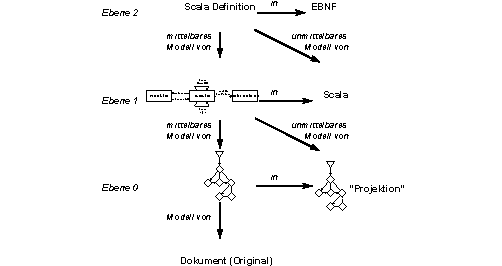
\includegraphics[width=1.45\textwidth]{figures/metamodellschema.svg.pdf} }
\caption{ Übersicht der Zusammenhänge des Dokumentmodells und Dokumentmetamodells. Grafik nach (Strahringer, 1998). Die erweiterte Backus-Naur-Form (EBNF) kann als Metametamodell dienen -- denn mit EBNF können Programmiersprachen beschrieben werden und zudem ist EBNF in der Lage sich selbst zu beschreiben. }\label{metamodellschema}
\end{figure}
 
\section{Semiotik}\label{}
 
\begin{quote}
 Semeiotik [sic] ist eigentlich nichts anderes als die allgemeine Lehre von den Sprachen. Ob diese nun künstliche oder natürliche Sprachen sind, spielt keine Rolle. \citep[S.~8]{Malissa}
\end{quote}
 
Die Gesetzmäßigkeiten einer Sprache kann allgemein in vier Hauptteile gegliedert werden, vgl. \citep[S.~8]{Malissa}:

 
\begin{enumerate}[(i)]

\item
Syntax (Struktur): Beschreibt die Beziehung zwischen Zeichen, Signalen, Symbolen zueinander. Hier kann man sich die Frage stellen: Was ist ein korrekter Aufbau eines Symbols? Zum Beispiel wenn man einen Satz einer natürlichen Sprache als Symbol ansieht, wird ein Satz nur durch eine bestimmten Reihung von Wörtern korrekt.


\item
Semantik (Bedeutung): „ist die Lehre von den Zeichen, Signalen, Symbolen und deren Bedeutung.“ (ebd.) Sie stellt also die Beziehung zwischen Symbol und des bezeichneten Objekts her. Hier kann man sich die Frage stellen: Was bedeutet das Symbol? Was ist die Bedeutung?


\item
Pragmatik (Funktion): Stellt die Beziehung zwischen Zeichen, Signalen, Symbolen und dem Sender bzw. Empfänger dar. Hier kann man sich die Frage stellen: Was ist der Zweck des Symbols? An wen ist es wozu gerichtet?


\item
Sigmatik (Bezeichnung): „stellt die Beziehung zwischen den Zeichen, Symbolen, Signalen usw. und dem, was sie bezeichnen her.“ (ebd.) Hier kann man sich die Frage stellen: Was bezeichnet das Symbol? Was ist das Bezeichnete?


\end{enumerate}
 
Wenn ein Zeichen, Signal, Symbol, etc. alle der oben genannten vier Aspekte aufzeigt, dann spricht man von einer Information. Im Allgemeinen sind diese vier Aspekte also die Grundlage jeder Information. In Abb. \ref{semiotik} sind die Aspekte anhand von Beispielen aus der analytischen Chemie visualisiert.

 
\begin{figure}[h!]
\centering
\advance\leftskip-2.5cm
\fbox{ 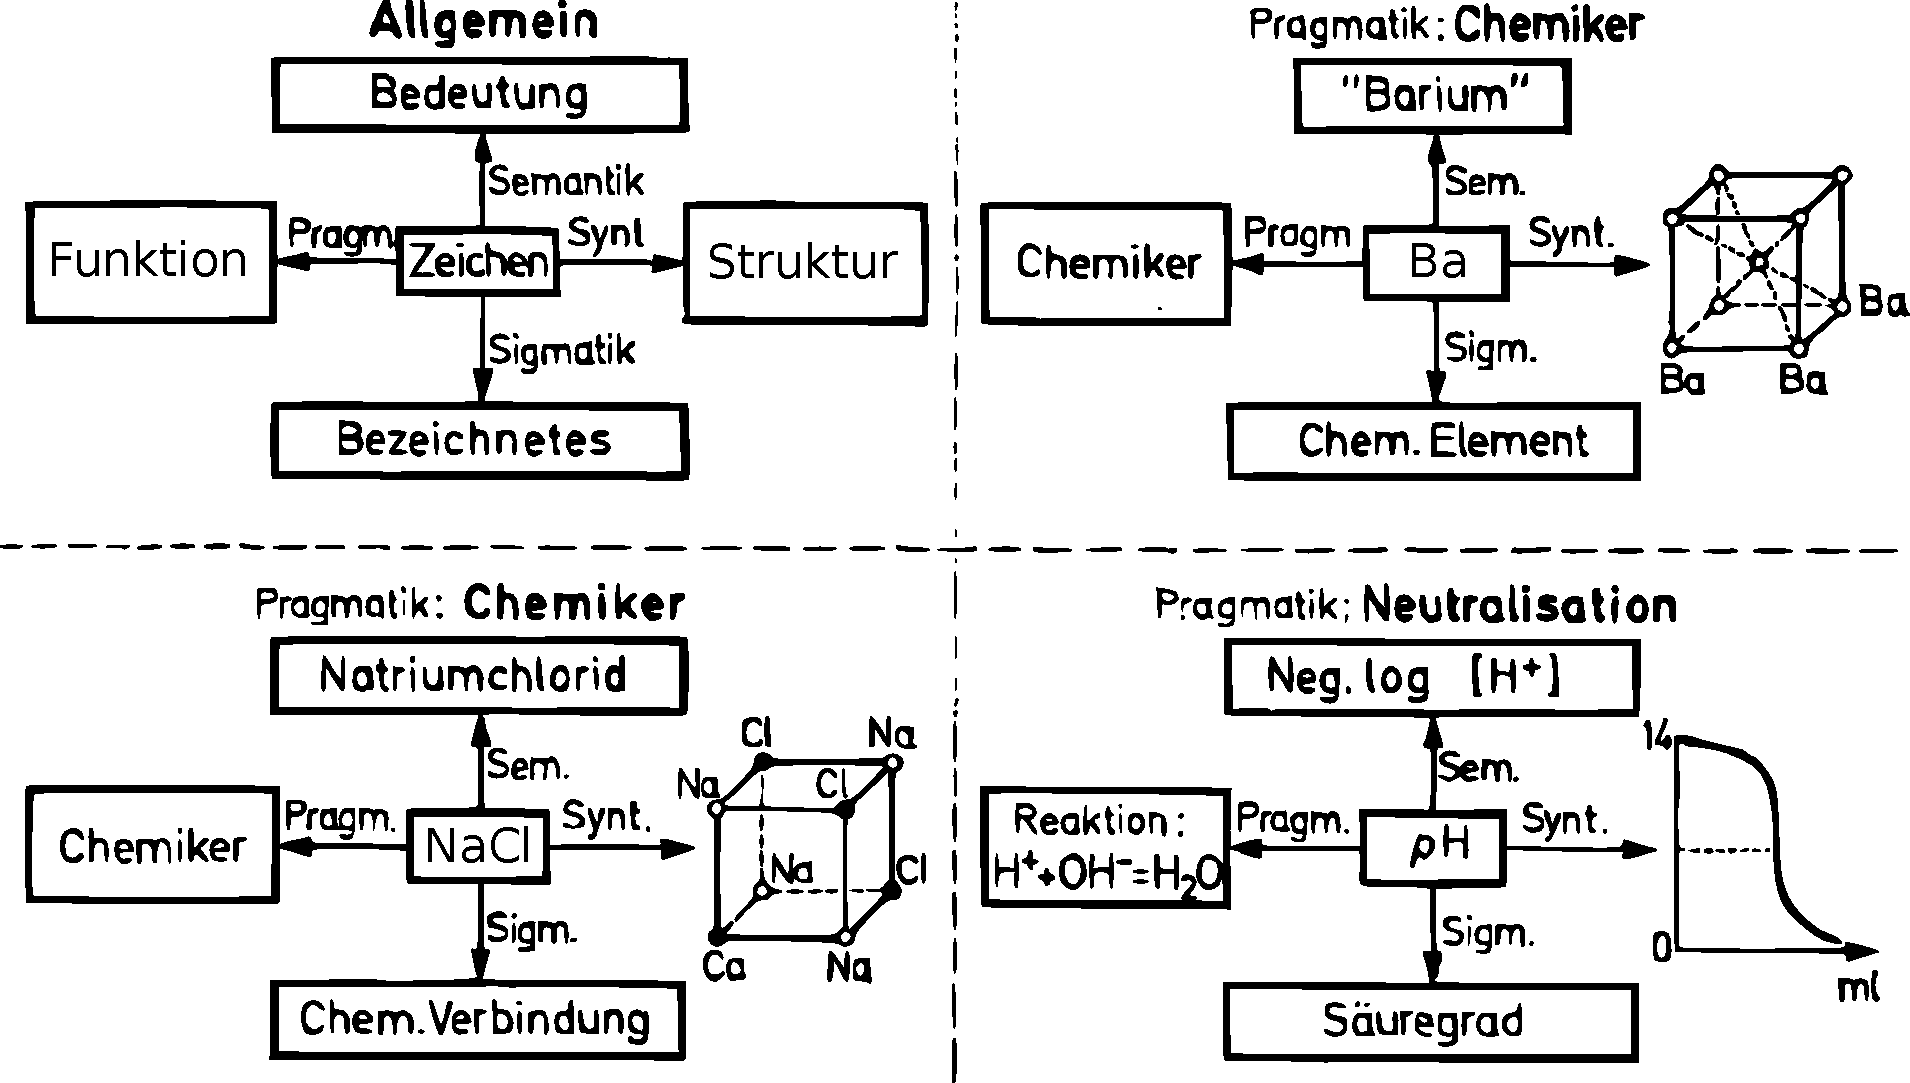
\includegraphics[width=1.45\textwidth]{figures/semiotik.svg.pdf} }
\caption{ Die vier Hauptteile der Semiotik grafisch dargestellt mit Beispielen aus der analytischen Chemie. Visualisierung mit einigen Anpassungen aus (Malissa, 1971, S. 9). }\label{semiotik}
\end{figure}
 
\subsection{Anwendung auf (wiss.) Dokumente}\label{}
 
Diese vier Aspekte kommen auch implizit in jedem Text zum tragen, da insb. wiss. Dokumente ein klassischer Informationsträger sind. In der Wissenschaft ist es üblich mit Modellen zu arbeiten. Diese Modelle sollen von anderen Wissenschaftlern möglichst leicht verstanden und benutzt werden. Für das Verstehen eines Modells ist es unerlässlich, die Bedeutungen jedes einzelnen Aspekts des Modells zu erfassen. Damit ein Leser einfach und gezielt Wissen aus dem Dokument ziehen kann, wäre es sicher nützlich, wenn diese Semantik möglichst explizit zur Verfügung stünde. Die Mechanik dazu könnte folgendermaßen aussehen: „Man fährt mit dem Mauszeiger über ein interessantes Objekt und erhält sofort weitere Informationen dazu, um mehr über die Bedeutung des Objektes zu erfahren.“

 
Wenn man die vier Konzepte allgemein auf den hier vorgestellten Prototypen übertragt, stellt man fest wie sich die Konzepte innerhalb eines Dokuments auswirken. Betrachtet wird ein einzelnes Dokumentelement:

 
\begin{itemize}

\item Zeichen: Entspricht einer Projektion des abstrakten Syntaxbaumes (z.B. ein Abschnitt-Dokumentelement gesetzt als „Kapitel 1. Einleitung“)
\item Bezeichnetes: Ist ein Dokumentelement.
\item Bedeutung: Erster gliedernder Abschnitt des Dokuments.
\item Funktion: Der Autor fungiert während des Schreibens als Sender und Empfänger.
\item Struktur: Entspricht dem abstrakten Syntaxbaum selbst bzw. dessen Metamodell.
\end{itemize}
 
Man kann argumentieren, dass hinter jedem Dokumentelement (z.B. Abschnitt, Absatz, Tabelle, ...) ein entsprechendes Domänenmodell steckt. Beispielsweise hinter einem Chemie-Dokumentelement stecke ein Moleküleditor, der ein entsprechendes Modell eines Moleküls produziert, sowie eine grafische Repräsentation (Bild eines Moleküls). Idealerweise liegt das Domänenmodell als domänenspezifische Sprache (DSL) vor. Im Bezug auf das Chemie-Dokumentelement könnte das die IUPAC-, Molfile- oder SMILES-Molekülnotation sein. Das würde bedeuten, dass der hier vorgestellte Syntaxbegriff auch gleichzeitig das Domänenmodell vertritt.

 
Das heißt, dass bei der Erstellung eines Dokuments Dokumentelemente vom Autor entworfen werden können, welche Modelle der jeweiligen Wissenschaft enthalten können. Das ermöglicht dem Autor deutlich strukturierter, formaler und konsistenter an die Dokumentation seins Projektes heranzugehen. Zudem werden dem Leser dadurch explizite semantische Informationen bereitgestellt, welche direkt vom dahinterstehenden Modell stammen. Der Leser kann ggf. das Modell seines Kollegen in eigenen Dokumenten wiederverwenden. Vorteil hierbei wäre, dass weniger Fehler entstehen, da direkt auf die Gedanken (welche in das Modell gegossen wurden) des Original-Autors zurückgegriffen werden kann.

 
Üblicherweise gibt es unter Dokumentelementen Verweise. Zum Beispiel ein Absatz-Dokumentelement möchte auf die Molekülmasse des Chemie-Dokumentelements verweisen. Dann sieht die Semiotik folgendermaßen aus:

 
\begin{itemize}

\item Zeichen: „Die Molekülmasse ist 144 g/mol.“ (So angezeigt durch den Absatz)
\item Bezeichnetes: Chemie(molekül)-Dokumentelement. (Welches das Modell des Moleküls enthält)
\item Bedeutung: Masse von Koffein in Gramm pro Mol. (Interessantes Objekt wäre „144 g/mol“)
\item Funktion: Verweis
\item Struktur: „{ koffein.masse }“ (hieraus folgt „144 g/mol“)
\end{itemize}
 
Mechanik: Der Programmierausdruck „koffein.masse“ (koffein wäre der Name des Chemie-Dokumentelements und masse eine bereitgestellte Methode des Chemie-Dokumentelement-Objektes) liefert ein semantisches Objekt, z.B. in Form eines Scala-Objekts des Typs Moleculemass. Moleculemass könnte mit den Properties mass, name, unit ausgestattet sein, um mehr Informationen über seine Bedeutung(en) bereitstellen zu können. Zudem könnte es noch an eine SI-Einheiten-Onologie angekoppelt sein, um die semantischen Informationen mit dem Semantic Web zu teilen. Wenn der Leser mit seinem Mauszeiger über „144 g/mol“ fährt, kann diese Information aus dem Moleculemass-Objekt geholt werden und in Form einer farbigen Annotation angezeigt werden.

 
\section{Taxonomie wissenschaftlicher Publikationen}\label{}
 
Über die Jahrhunderte in denen wissenschaftliche Texte verfasst wurden, haben sich gewisse Konventionen und Vorgehensmodelle, wie ein Dokument von seinem inneren Aufbau her beschaffen sein soll, herauskristallisiert. Diese Konventionen haben sich sogar über nationale Grenzen hinweg sehr ähnlich entwickelt, was es der Wissenschaftsgemeinde leichter macht, ihr intellektuelles Vermächtnis zu teilen.

 
In Recherchen ist aufgefallen, dass es schon (wenn auch wenige) Versuche gegeben hat, eine möglichst allgemeingültige Systematik (z.T. formal) des inneren Dokumentenaufbaus herauszudestillieren. Jedoch sind diese Konzepte bisher kaum verbreitet, insbesondere bei der direkten Erstellung von (wiss.) Texten durch den Autor. Heutigen Autorensysteme unterstützen kaum explizite Semantik über das Domänenwissen mit dem sie gerade arbeiten -- dies fördert Fehler und Inkonsistenzen im Dokument.

 
Die DIN-Normen \citep{DIN1421}, \citep{DIN1422-1}, \citep{DIN1422-3} und \citep{DIN1422-4} geben Empfehlungen, wie Texte gegliedert und benummert werden sollen bzw. wie im allgemeinen Manuskripte oder Forschungsberichte gestaltet werden sollen. Dies sind keine formalen Vorgaben, sondern vielmehr eine Zusammenfassung der hiesigen guten fachlichen Praxis in Wissenschaft, Technik, Wirtschaft und Verwaltung. Anders hingegen geht \citep{NISO} vor, hier wird formal mittels XML Schemas eine allgemein gültige Menge an XML-Tags für den Aufbau von Fachzeitschriftenartikeln zusammengestellt. Jedoch haben diese auch für anderen Publikationen ihre Gültigkeit, wie z.B. Briefe, Leitartikel oder Buchkritiken. \citep{Peroni} stellt eine Ontologie (in OWL 2) über einzelnen Komponenten, die in einem Dokument vorkommen können, zur Verfügung. Hier werden die Beziehungen die die Komponenten untereinander pflegen sichtbar gemacht. Es wird dabei zwischen strukturierenden (z.B. Abschnitt, Absatz) und rhetorischen Komponenten (z.B. Einleitung, Abbildung, Anhang) unterschieden.

 
Hier soll versucht werden die Erkenntnisse der o.g. Quellen zu generalisieren, in der Hoffnung die Basis für ein formaleres bzw. präskriptiveres Autorensystem zu schaffen.

 
\subsection{Dokumentelemente}\label{dokumentelemente}
 
Dokumentelemente bilden das Grundgerüst eines jeden Dokuments. Hier wird versucht den Begriff genauer zu fassen und zu definieren. Es ergeben sich drei abstrakte Ausprägungen der Dokumentelemente:

 
\begin{itemize}

\item Struktur Elemente: Repräsentieren Komponenten, die textuellen bzw. grafischen Inhalt des Dokuments beinhalten. Sie tragen maßgeblich zum gedanklichen Gebäude des Dokuments bei.
\item Container Elemente: Beinhalten andere Dokumentelemente (als Kinder), und haben daher für gewöhnlich keine Repräsentation die aktiv zum eigentlichen intellektuellen Inhalt des Dokuments beiträgt. Sie gruppieren also Elemente zu größeren Dokument-Bestandteilen; dies gibt Vorteile bei der Verarbeitung und Semantik des Dokuments. Beispielsweise werden Dokumente oft in Titelei und Hauptteil unterteilt, wobei die Titelei gerne römisch nummeriert wird und der Hauptteil arabisch. Hat man hier eine explizite Hierarchievorgabe zur Hand, erleichtert das die Verarbeitung; wie im Beispiel die gewollten Nummerierungskonventionen durchzusetzen.
\item Metadaten Elemente: Sind Elemente die andere Elemente beschreiben bzw. allgemein gesprochen enthalten sie Daten über Daten. Beispielsweise eine Literatureintrag beschreibt lediglich einen Original-Artikel; oder eine Fußnote enthält eine Anmerkung über ein anderes Dokumentelement (die Fußnote verändert den Inhalt den das Dokument transportieren will an sich nicht, aber sie macht ihn verständlicher).
\end{itemize}
 
Die Dokumentelemente können zudem auch noch Attribute oder Properties enthalten. Diese enthalten Fakten über das betreffende Element, z.B. ob es sich bei einer Liste um eine geordnete Liste oder ungeordnete Liste handelt. Im Falle des hier vorgestellten Prototypen, kann man argumentieren, dass in den Attributen auch das jeweils vorliegende Domänenmodell des Dokumentelements abgelegt wird.

 
In DoCO wird ein Unterschied zwischen strukturierenden (z.B. Abschnitt, Absatz) und rhetorischen Komponenten (z.B. Einleitung, Diskussion, Abbildung) unterschieden. Hier wird jedoch nur das Struktur Element benötigt, da die rhetorische Bedeutung über die Attribute des Elements hinzugefügt werden kann. Allgemein gesprochen gehört die rhetorische Bedeutung zur Semantik des Elements. Die Semantik des Elements wird wiederum maßgeblich über das Domänenmodell gewonnen und dieses ist wiederum in den Attributen ansässig. Daher muss kein Unterschied zwischen strukturierenden und rhetorischen Komponenten gemacht werden.

 
\subsubsection{Bedeutung für das Dokumentmodell}\label{}

 
Im Dokumentmodell, also dem abstrakten Syntaxbaum entsprechen die Struktur Elemente den Blättern und die Container Elemente entsprechen den inneren Knoten. Metadaten Elemente kommen entweder wie Struktur Elemente vor oder werden in ein extra „Metadokument“ ausgelagert, falls die Metadaten Elemente nur einzelne Attribute bereitstellen sollen und nicht in Gänze angezeigt werden.

 
\subsubsection{Verweisungen}\label{}

 
\citep{Peroni} und \citep{NISO} modellieren mehr Dokumentelemente als in der vorgestellten Taxonomie (s. Abschnitt \ref{taxonomiesec}). Das liegt zum einen daran, dass hier viele dieser „Elemente“ in dem hier vorgestellten Modell als Attribute abgelegt werden. Hier treten nur die Komponenten explizit als Dokumentelement auf, bei denen es Sinn macht auch als ein Knoten des abstrakten Syntaxbaumes abgebildet zu werden. Zum anderen werden in den Modellen von (ebd.) Verweisungen, die sich innerhalb des Dokuments abspielen (z.B. auf Kapitel oder Abbildungen), auch explizit als Dokumentelement modelliert. Dies macht aber in dem hier vorgestellten Dokumentmodell wenig Sinn.

 
Denn hier treten Verweisungen nicht in Form von Knoten auf, sondern sie entsprechen den Kanten des Dokumentengraphs. Wenn ein Knoten (also Dokumentelement) eine Information von einem anderen Knoten erhalten will, werden Nachrichten mit den Informationen ausgetauscht. Durch diesen Mechanismus werden die Verweisungen im Dokument schlussendlich aufgelöst. Wir haben also ein ganz klares Modell: Inhalte in die Blätter, Hierarchie in die inneren Knoten, Semantik und Modelle in die Attribute und Verweisungen fließen über die Kanten, also in der Implementierung des Prototypen als Nachrichten-Kommunikation.

 
\subsection{Taxonomie}\label{taxonomiesec}
 
In der Tabelle auf Abb. \ref{taxonomie} sind nochmals alle drei Ausprägungen der Dokumentelemente (s. Abschnitt \ref{dokumentelemente}) übersichtlich dargestellt. Sie sind von abstrakt zu konkreter werdend geordnet. In der vorletzten Spalte sind die eigentlichen Kernelemente aufgezeigt, welche auch so im Dokument vorkommen können. In der letzten Spalte sind mögliche Attribute, Properties bzw. Methoden aufgelistet, die dem Element zusätzliche (semantische) Informationen hinzufügen.

 
Mit den in der Tabelle (Abb. \ref{taxonomie}) aufgelisteten Dokumentelementen kann man ein typisches, aber sehr allgemein gehaltenes, wissenschaftliches Dokument aufbauen. Die Gesamtheit der hier vorliegenden Dokumentelemente beschreibt somit eine ganz bestimmte Dokumentklasse, welche als allgemeiner „wissenschaftlicher Bericht“ oder „Report“ bezeichnet werden kann. Aber es gibt auch noch beliebige andere Klassen (z.B. Patente, Normen, Softwaredokumentation, etc.), die möglicherweise einen (leicht) anderen Aufbau haben und somit ggf. andere Dokuementelemente benötigen. Neu definierte Dokumentelemente (z.B. für eine andere Dokumentklasse) sollten sich leicht in diese Taxonomie eingliedern lassen. Damit liegen sie nicht mehr als implizite Aufbauvorschrift (gemeint ist so etwas wie ein Corporate Design) vor, sondern sind explizit, für die Nutzung in einem Autorensystem welches die Taxonomie umsetzt, formalisiert.

 
\begin{figure}[h!]
\centering
\advance\leftskip-2.5cm
\fbox{ 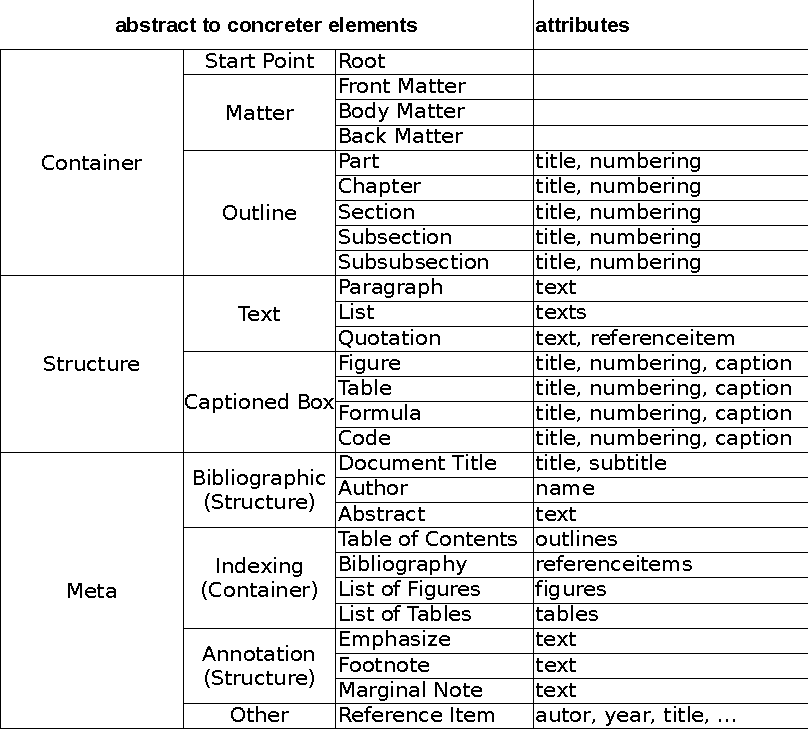
\includegraphics[width=1.45\textwidth]{figures/taxonomie.svg.pdf} }
\caption{ Taxonomie des inneren Aufbaus von wissenschaftlichen Dokumenten. Sortiert von abstrakt zu konkret. }\label{taxonomie}
\end{figure}
 
\subsection{Dokumentstruktur Matrix}\label{}
 
Damit das Autorensystem beim Erstellen eines formal korrekten Dokuments helfen kann, wird ein Regelwerk benötigt welches vorschreibt „welches Element nach wem erlaubt ist“ (erlaube Geschwister-Beziehungen) und „wo darf welches Element vorkommen“ (erlaube Eltern-Kind-Beziehungen).

 
Durch diese Formalisierung kann der Autor wie auf Schienen durch den Aufbau geführt werden.Er muss sich also nicht mehr selbst darum kümmern die impliziten Vorgaben der Dokumentklasse durchzusetzen.Das heißt er macht weniger Fehler beim Aufbau des Dokuments, da das System assistierend zur Seite steht, um die gewählte Dokumentklasse ihrem Regelwerk konform zu halten und er sich stärker auf die Erstellung des Inhalt konzentrieren kann.Zudem liefert jedes Dokumentelement ein Set an Attributen mit, was es ermöglicht mehr explizite Semantik in das Dokument zu bringen und das Dokument insgesamt konsistenter zu halten.

 
\subsubsection{Erlaube Verschachtelungen}\label{}

 
Auf Abbildung \ref{matrixkind} sind die erlaubten Eltern-Kind-Beziehungen der vorliegenden Dokumentklasse definiert. Die hier dargestellte Matrix ist eine Vereinfachung, also nur eine Auswahl an Dokumentelementen, der Taxonomie aus Tabelle auf Abb. \ref{taxonomie}. Diese Matrix definiert die erlaube Schachtelung der vorliegenden Dokumentklasse.

 
\begin{figure}[h!]
\centering
\advance\leftskip-2.5cm
\fbox{ 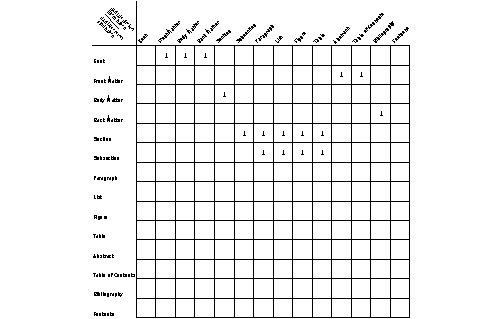
\includegraphics[width=1.45\textwidth]{figures/matrixkind.svg.pdf} }
\caption{ Stellt die erlaubten Eltern-Kind-Beziehungen zwischen den Dokumentelementen dar. Hier wird also definiert mit welchen Elementen die Hierarchie des Dokuments aufgespannt werden darf. }\label{matrixkind}
\end{figure}
 
\subsubsection{Erlaube Abfolgen}\label{}

 
Auf Abbildung \ref{matrixgeschwister} sind die erlauben Nachfolger-Vorgänger-Bezeihungen der hier beispielhaft vorliegenden Dokumentklasse als Matrix dargestellt. Hier wird also die Frage geklärt, welches Dokumentelemente aneinander gereiht werden dürfen, um ein wohlgeformtes Dokument der vorliegenden Dokumentklasse zu bilden.

 
\begin{figure}[h!]
\centering
\advance\leftskip-2.5cm
\fbox{ 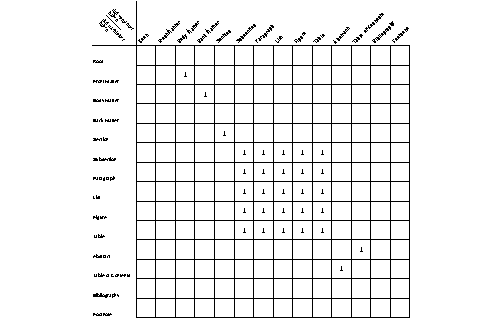
\includegraphics[width=1.45\textwidth]{figures/matrixgeschwister.svg.pdf} }
\caption{ Stellt die erlaubten Geschwister-Beziehungen (Nachfolger/Vorgänger) zwischen den Dokumentelementen dar. Hier wird also definiert welche Elementen aneinandergereiht werden dürfen. }\label{matrixgeschwister}
\end{figure}
 
\subsection{Deutung}\label{}
 
Wenn man also ein Set an Dokumentelementen definiert und in die Taxonomie eingegliedert hat, zudem noch die erlaubten Beziehungen zwischen den Dokumentelementen in Matrixform definiert hat, dann erhält man eine präzise definierte Dokumentklasse. Nützlich ist das nicht nur um dem Autor „Schienen“ für die Dokumenterstellung bereitzustellen, sondern auch für Klassifikationsaufgaben. Beispiel: Im Zuge von Information Retrieval hat man verschiedene mit OCR aufbereitete PDFs, welche man gerne einer Dokumentklasse zuordnen möchte, um sie wieder in ein „sauberes“ oder aktuelles Template zu überführen. Wenn nun ein Klassifikator die aufbereiteten PDFs in ihre Dokumentelemente zerlegt, kann über die Gesamtheit der im PDF gefunden Dokumentelemente und deren Anordnung bzw. Verschachtelung, dank der aufgestellten Taxonomien bzw. Matrizen, auf die Dokumentklasse (z.B. EU-Patent, US-Patent, DIN-Norm, etc.) zurückgeschlossen werden.
